\begin{enumerate}[\Large\bfseries 1.]

%--------------------1.
\item \textbf{\large Desigualdades que relacionan distintos tipos de promedios}\\\\

    \begin{enumerate}[\bfseries a)]

	%----------a.
	\item \textbf{(Tom Apostol, Calculus Vol 1)}\\\\ Sean $x_1,x_2,...,x_n$ $n$ números reales positivos. Si $p$ es un entero no nulo, la media de potencias p-énesimas $M_p$ se define como sigue.
$$M_p = \left( \dfrac{x_1^{p} + ... + x_{n}^{p}}{n} \right)^{1/p}$$
El número $M_1$ se denomina media aritmética, $M_2$ media cuadrática y $M_{-1}$ media armónica.\\\\

	%----------b)
	\item \textbf{Código fuente.}\\ 
	    
	    \lstinputlisting[language=Python]{python/tareas_mat/week3/promedios.py}
	    \vspace{.5cm}
	
	%----------c)
	\item \textbf{Prueba de la ejecución del programa}.\\
	    \begin{center}
		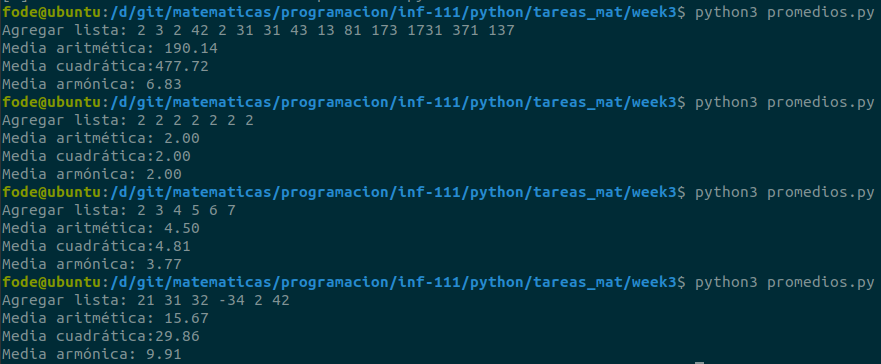
\includegraphics[scale=.4]{imagenes/tareas_mat/week3/promedios.png}
	    \end{center}

    \end{enumerate}

\newpage

%--------------------2.
\item \textbf{\large Obtención de las estimaciones de mínimos cuadrados ordinarios}\\\\

    \begin{enumerate}[\bfseries a)]

	%----------a.
	\item \textbf{(George Wooldridge, Introducción a la econometría, capítulo 2)}.\\\\ Sea $\left\{(x_i,y_i): i = 1,\ldots,n\right\}$, una muestra aleatoria de tamaño $n$ tomada de la población. Como estos datos provienen de $(2.1)$ para todo $i$ puede escribirse 
\begin{equation}
    y_i = \beta_o + \beta_1x_i + u_i.
\end{equation}

En tanto el intercepto $\beta_0$ aparezca en la ecuación, nada se altera al suponer que el valor promedio de $u$ en la población, es cero. Es decir, $E(u)=0$.\\
El supuesto crucial es que el valor promedio de $u$ no depende del valor de $x$. Este supuesto se expresa como $u$ $E(u\backslash x) = E(u)$. Esta última ecuación indica que el valor promedio de los factores no observables es el mismo en todas las fracciones de la población determinados por los valores de $x$ y que este promedio común es necesariamente igual al promedio al promedio de $u$ en toda la población. Y por lo tanto $u$ es media independiente de $x$. Combinando la independencia de la media con el supuesto de $E(u)=0$ se obtiene el supuesto de media condicional cero, $E(u\backslash x) = 0$\\\\

En la población, $u$ no está correlacionada con $x$. Por tanto, se tiene que el valor esperado de $u$ es cero y que la covarianza entre $x$ y $y$ es cero:
\begin{equation}
    E(u)=0
\end{equation}
 y 

\begin{equation}
    Cov(x,u) = E(xu) =0.
\end{equation}

\textbf{Covarianza.-} Sean $\mu_x = E(X)$ y $\mu_y = E(Y)$ y considere la variable aleatoria $(X-\mu_x)(Y-\mu_y)$. Si $X$ es mayor a su media y $Y$ es mayor a su media, entonces $(X-\mu_x)(Y-\mu_y)>0$. La covarianza entre dos variables aleatorias $X$ y $Y$ llamada algunas veces covarianza poblacional, para hacer énfasis en que se refiere a la relación entre dos variables que describen una población, está definida como el valor esperado del producto $(X-\mu_x)(Y-\mu_y)$: 

\begin{equation}
    Cov(X,Y) = E\left[(X-\mu_x)(Y-\mu_y)\right]
\end{equation}

que también suele denotarse como $\sigma_{XY}.$  \\
Algunas expresiones para útiles para calcular $Cov(X,Y)$ son las siguientes

\begin{equation}
    Cov(X,Y) = E\left[(X-\mu_x)(Y-\mu_y)\right] = E\left[(X-\mu_X)Y\right] = E\left[X(Y-\mu_Y)\right] = E(XY) - \mu_x \mu_y
\end{equation}

De donde se sigue que si $E(x)=0$ o $E(Y)=0$, entonces $Cov(X,Y) = E(XY)$.\\\\

Luego  
\begin{equation}
    E(y - \beta_0 - \beta_1x) = 0
\end{equation}
 
y 

\begin{equation}
    E\left[x(y - \beta_0 -\beta_i x )= 0\right]
\end{equation}

Como hay que estimar dos parámetros desconocidos, se espera que las dos ecuaciones anteriores puedan servir para obtener buenos estimadores de $\beta_0$ y $\beta_1$. En efecto estas ecuaciones pueden servir para la estimación de estos parámetros.\\\\

Por el método de momentos para la estimación , y las anteriores dos ecuaciones,
\begin{equation}
    n^{-1} \sum\limits_{i=1}^n (y_i - \beta_0 - \beta_1x_i) = 0
\end{equation}
y 
\begin{equation}
    n^{-1} \sum\limits_{i=1}^n x_i(y_i - \beta_0 - \beta_1x_i) = 0
\end{equation}
Luego por la ecuación (2.9) tenemos que 
\begin{equation}
    \overline{y} = \hat{\beta_0} + \hat{\beta_1}\overline{x}.
\end{equation}
donde $\overline{y} = n^{-1}\sum\limits_{i=1}^n y_i$ es el promedio muestral de las $y_i$, y lo mismo ocurre con $\overline{x}$, así, 

\begin{tcolorbox}[colframe=white]
\begin{equation}
    \hat{\beta_0} = \overline{y} - \hat{\beta_1}\overline{x}.
\end{equation}
\end{tcolorbox}
Por último empleando (2.10) y (2.12) para sustituir $\hat{\beta_0}$ se obtiene,
$$\sum_{i=1}^n x_i\left[y_i-(\overline{y}-\hat{\beta_1}\overline{x})-\hat{\beta_1}x_i\right] = 0,$$
de donde, reordenando, tenemos que
$$\sum_{i=1}^n x_i(y_i-\overline{y}) = \hat{\beta_1}\sum_{i=1}^n x_i(x_i-\overline{x}).$$
en consecuencia por las propiedades de la sumatoria, 
$$\sum_{i=1}^n x_i(x_i-\overline{x}) = \sum_{i=1}^n (x_i-\overline{x})^2 \quad y \quad \sum_{i=1}^n x_i(y_i-\overline{y}) = \sum_{i=1}^n (x_i-\overline{x})(y_i-\overline{y})$$\\
ya que $$\sum\limits_{i=1}^n (x_i-\overline{x})(y_i-\overline{y})=\sum\limits_{i=1}^n x_i y_i - \overline{y}\sum\limits_{i=1}^n x_i - \overline{x}\sum\limits_{i=1}^n y_i + \overline{y} \overline{x}\sum\limits_{i=1}^n 1,$$ luego ya que $\sum\limits_{i=1}^n x_i = n\overline{x}$ entonces $$\sum\limits_{i=1}^n x_iy_i - n\overline{yx} - n\overline{xy} + n\overline{xy} = \sum\limits_{i=1}^n (x_i-\overline{x})y_i$$
por lo tanto, 
\begin{tcolorbox}[colframe=white]
\begin{equation}
    \hat{\beta_1} = \frac{\sum\limits_{i=1}^n (x_i-\overline{x})(y_i-\overline{y})}{\sum\limits_{i=1}^n (x_i-\overline{x})^2}.
\end{equation}
\end{tcolorbox}
Ésta ecuación no es nada mas que la covarianza muestral en $x$ e $y$ dividida entre la variación muestral de $x$.

\newpage

	%----------b)
	\item \textbf{Código fuente.}\\ 
	    
	    \lstinputlisting[language=Python]{python/tareas_mat/week3/MCO.py}
	    \vspace{1cm}
	
	%----------c)
	\item \textbf{Prueba de la ejecución del programa}.\\
	    \begin{center}
		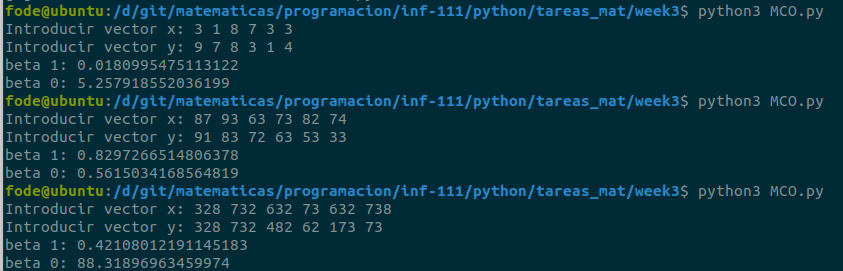
\includegraphics[scale=.5]{imagenes/tareas_mat/week3/MCO.png}
	    \end{center}

    \end{enumerate}

\newpage


%--------------------3.
\item \textbf{VARIANZA}\\\\

    \begin{enumerate}[\bfseries a)]

	%----------a.
	\item \textbf{Fórmula}\\\\ 
	    $$Var(x) = \dfrac{\sum\limits_{i=1}^{n} (x_i - \overline{X})^2}{n}$$\\\\

	%----------b)
	\item \textbf{Código fuente.}\\ 
	    
	    \lstinputlisting[language=Python]{python/tareas_mat/week3/var.py}
	    \vspace{3cm}
	
	%----------c)
	\item \textbf{Prueba de la ejecución del programa}.\\
	    \begin{center}
		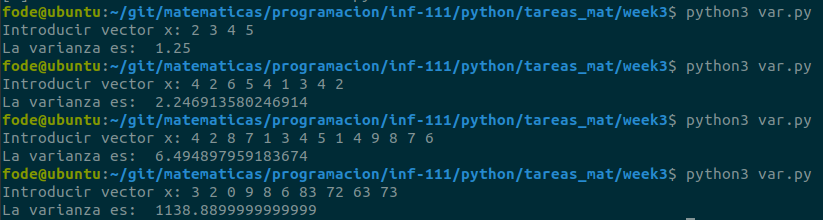
\includegraphics[scale=.5]{imagenes/tareas_mat/week3/var.png}
	    \end{center}

    \end{enumerate}

\newpage

%--------------------4.
\item \textbf{PRODUCTO ESCALAR}\\\\

    \begin{enumerate}[\bfseries a)]

	%----------a.
	\item \textbf{Definición}\\\\ 
	    Si $A=\lbrace a_1,\ldots a_n\rbrace$ y $B=\lbrace b_1,\ldots, b_n\rbrace$ son dos vectores de $V_n$ su producto escalar se representa con $A\cdot B$ y se define con la igualdad,
	    $$A\cdot B = \sum_{k=1}^n a_k b_k$$\\\\

	%----------b)
	\item \textbf{Código fuente.}\\ 
	    
	    \lstinputlisting[language=Python]{python/tareas_mat/week3/prod_escalar.py}
	    \vspace{3cm}
	
	%----------c)
	\item \textbf{Prueba de la ejecución del programa}.\\
	    \begin{center}
		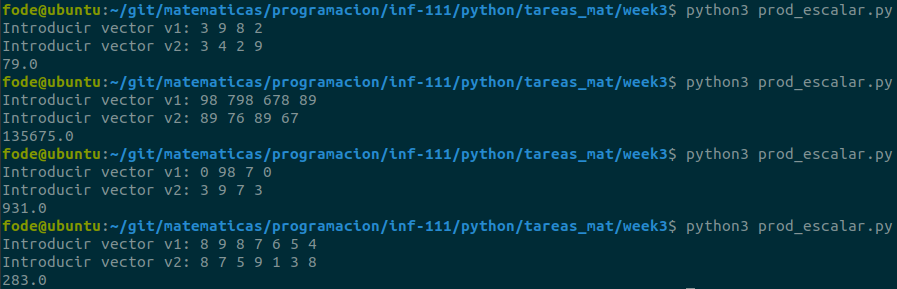
\includegraphics[scale=.5]{imagenes/tareas_mat/week3/escalar.png}
	    \end{center}

    \end{enumerate}

\newpage

%--------------------5.
\item \textbf{NORMA DE UN VECTOR}\\\\

    \begin{enumerate}[\bfseries a)]

	%----------a.
	\item \textbf{Definición}\\\\
	    Si $A$ es un vector de $V_n$, su longitud o norma se designa con $\|A\|$ y se define mediante la igualdad $$\|A\| = (A\cdot A)^{1/2}$$\\\\

	%----------b)
	\item \textbf{Código fuente.}\\ 
	    
	    \lstinputlisting[language=Python]{python/tareas_mat/week3/norma.py}
	    \vspace{3cm}
	
	%----------c)
	\item \textbf{Prueba de la ejecución del programa}.\\
	    \begin{center}
		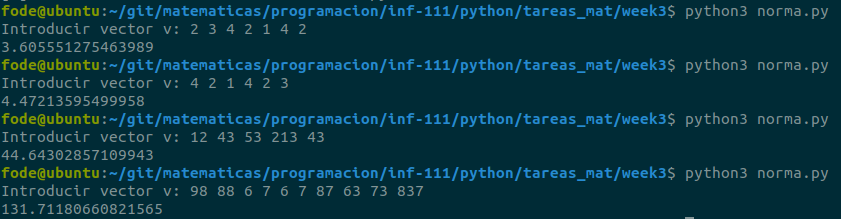
\includegraphics[scale=.5]{imagenes/tareas_mat/week3/norma.png}
	    \end{center}

    \end{enumerate}

\newpage
\end{enumerate}
